\documentclass[Proceedings]{ascelike}
%
% Feb. 14, 2013
%
% Some useful packages...
%
\usepackage{graphicx}
\usepackage{float}
%\usepackage{cite}
\usepackage{cleveref}
%\usepackage{subfigure}
%\usepackage{amsmath}
%\usepackage{amsfonts}
%\usepackage{amssymb}
%\usepackage{amsbsy}
%\usepackage{times}
%
%
% Place hyperlinks within the pdf file (works only with pdflatex, not latex)
% \usepackage[colorlinks=true,citecolor=red,linkcolor=black]{hyperref}
%
%
% NOTE: Don't include the \NameTag{<your name>} if you have selected 
%       the NoPageNumbers option: this leads to an inconsistency and
%       a warning, and the NameTag is ignored.
%
%
\begin{document}
%
% You will need to make the title all-caps
\title{On Neural Network Initialization}
%
\author{
Vivek Rathod, Guifan Li
}
%
\maketitle
%

\Section{abstract}
This is a report describing the experimental results on the performance of a shallow neural network on MNIST digits dataset with different weight initialization schemes.
\section{Network Structure}
\label{sec:network_struct}
We built a shallow neural network with one hidden layer with $tanh$ activation units as recommended in \cite{lecun2012efficient} \[1.7159*\tanh\left(\frac{2}{3}x\right)\] and an output layer with $softmax$ activation units to model the problem as a multinomial classification problem:\[P(y=j|x)=\frac{e^{x^{T}w_j}}{\sum_{k=1}^Ke^{x^{T}w_k}}\] The input layer has $784$ units and the output layer has $10$ units corresponding to the ten target classes. All the units in each layer are fully connected. 

\Section{Training method}
\label{sec:train_method}
The neural Network is trained using mini-batch stochastic gradient descent (SGD) back propagation with a batch size of 32. A constant learning rate of $0.01$ is used. SGD is run for a fixed number of iterations and the model that performs best on the validation set at any time during training is used as the final model. 

\Section{Weight Initialization}
\label{sec:weight_init}
Neural Networks are commonly initialized with weights sampled randomly from a uniform distribution such that the network begins operating in its linear regime. This ensures that the gradients are large enough when the training begins. In addition, it also helps the network to learn the linear features first and harder non-linear features next. Weights at each layer are initialized at each layer using the following heuristic: 
\[W_{ij} = U\left[-\frac{1}{\sqrt{n}},\frac{1}{\sqrt{n}}\right]\] where $U[-a, a]$ is the uniform distribution in the interval $(-a, a)$ and $n$ is the size of the previous layer ~\cite{erhan2009difficulty}. The biases are set to zero or initilized from the same uniform distribution as the weights.

\Section{Experiments}
We performed several experiments with the shallow neural network and MNIST digits dataset. The mnist training data set is split into two--- a set of $50000$ examples is used for training set and and the set of other $10000$ examples is used for the validation. The standard mnist test set is used for testing the performance of the neural network. The dataset is standardized to have a mean of zero and variance of one in all features.
\subsection{Shallow Neural Network}
We set up a shallow neural network as described in section ~\ref{sec:network_struct} with $300$ hidden units. The weights were initialized as described in section ~\ref{sec:weight_init}. The network was trained with mini-batch SGD back propagation. The network converges to zero error after $30$ passes through the dataset and achieves an error of $0.036$ on the test set. The Training and Validation errors over training epochs are show in figure ~\ref{fig:sn_test_err}. We also plot the distribution of weights and biases to  monitor the change over training epochs in figure \ref{fig:wt_dist}. Finally figure ~\ref{fig:actv_dist} shows the distribution of activations that units in hidden layer output. 


\begin{figure}[H]
  \caption{Training and Validation Error}
  \label{fig:sn_test_err}
  \centering
  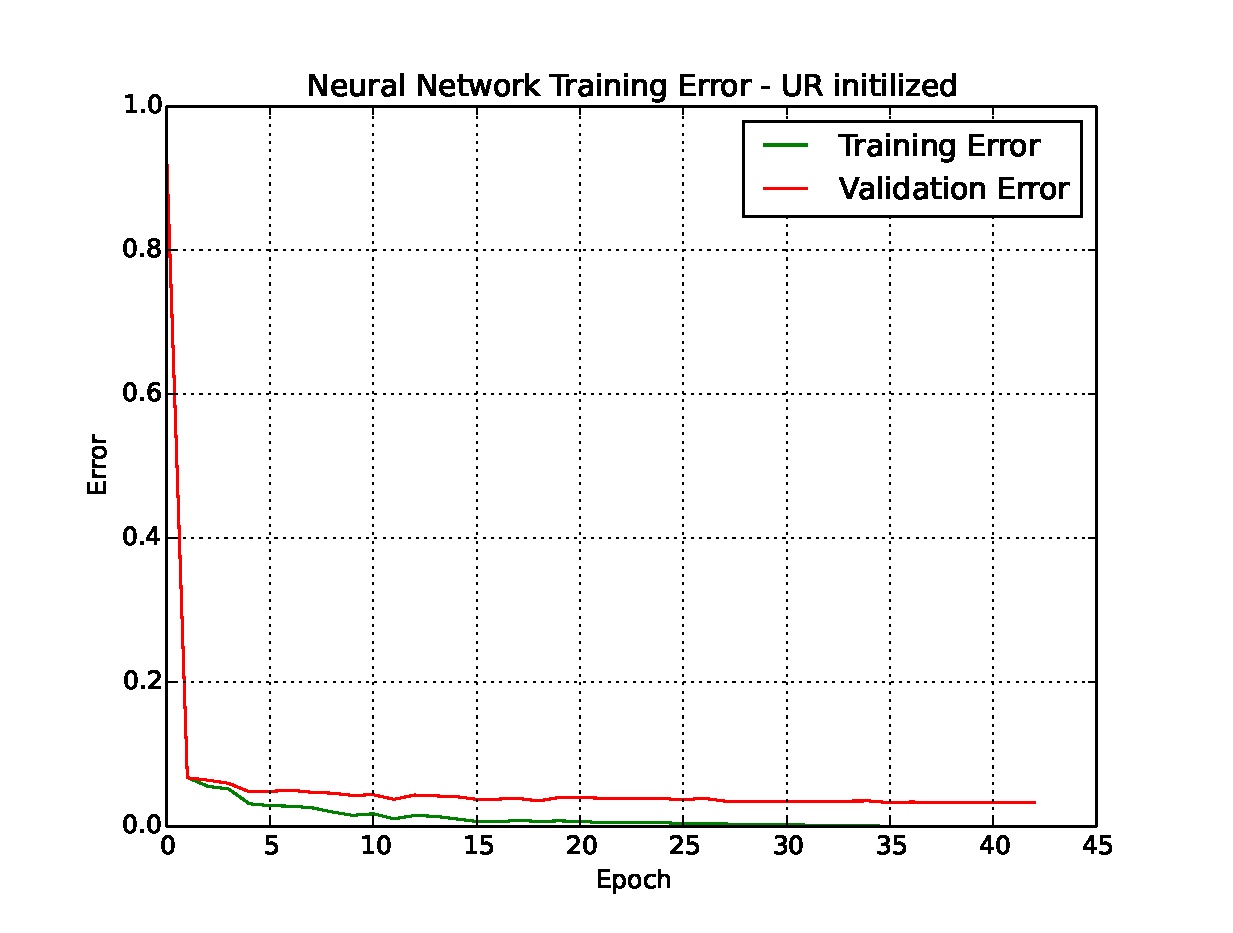
\includegraphics[width=0.7\textwidth, keepaspectratio]{shallownet_perf.eps}
\end{figure}

\begin{figure}[H]
  \caption{Weight Distribution}
  \label{fig:wt_dist}
  \centering
  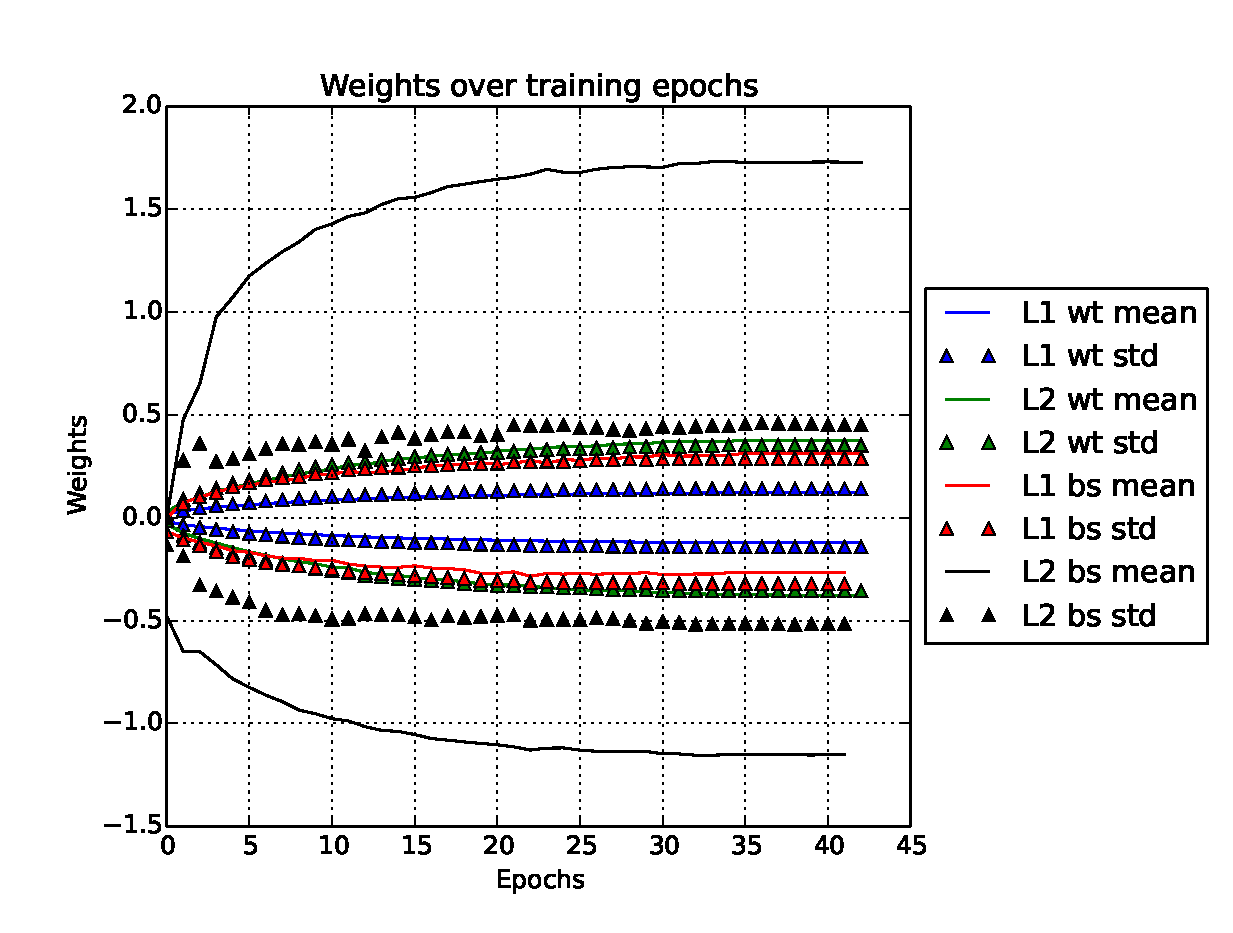
\includegraphics[width=0.7\textwidth, keepaspectratio]{shallownet_weights.eps}
\end{figure}

\begin{figure}[H]
  \centering
  \label{fig:actv_dist}
  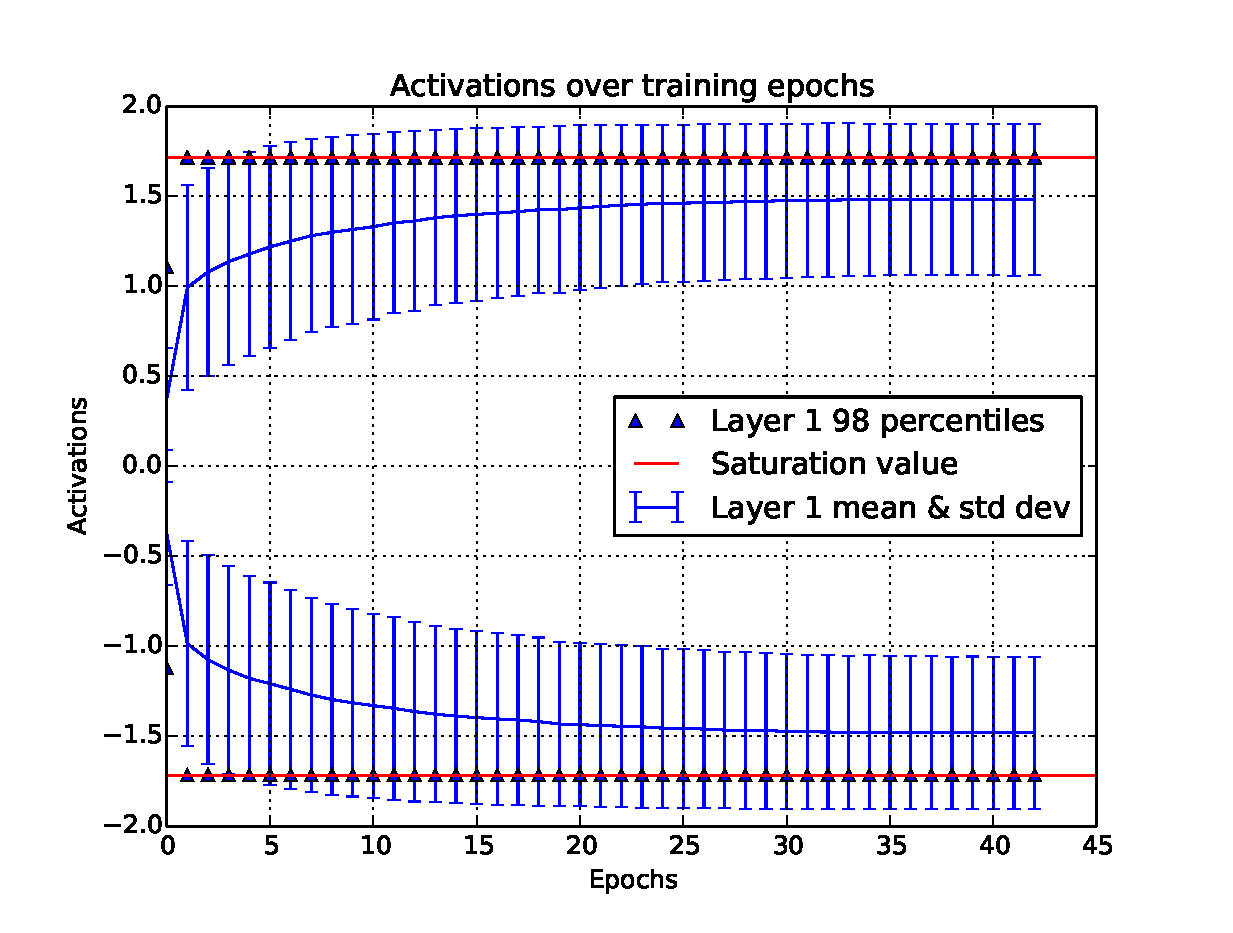
\includegraphics[width=0.7\textwidth, keepaspectratio]{shallownet_actv.eps}
   \caption{Layer 1 Activations}
\end{figure}


\subsection{Random Features Network}
We performed an experiment to determine the performance of neural network with random (linear and non linear) features. This is done by keeping the weights that map the input layer to the hidden layer (IHL) fixed, while changing only the weights that map the hidden layer to the output layer (HOL) using Back Propagation. The weights in HOL initialized as mentioned in section~\ref{sec:weight_init} while the weights in IHL are sampled randomly from a uniform distribution $U[-a, a]$ where $a$ is varied from $0.01$ to $3.0$. The hidden layer is set to have $300$ hidden units. The network is trained using back propagation for $10$ epochs with a fixed learning rate and batch size as mentioned in section~\ref{sec:train_method}. The error obtained on the test set is recorded in table~\ref{tab:terror}

\begin{table}[H]
\centering
\begin{tabular}{|c||c|}
\hline
$a$&$Test Error$\\
\hline
\hline
0.01&0.0885\\
0.035&0.0853\\
0.1&0.1072\\
0.3&0.129\\
0.9&0.1488\\
3.0&0.1554\\
\hline
\end{tabular}
\caption{Random Feature Shallow Network with 300 Hidden Units}
\label{tab:terror}
\end{table}

\bibliography{report.bib}{References}
\bibliographystyle{plain}

\end{document}

